% !TEX TS-program = XeLaTeX
% use the following command:
% all document files must be coded in UTF-8
\documentclass[spanish]{textolivre}
% build HTML with: make4ht -e build.lua -c textolivre.cfg -x -u article "fn-in,svg,pic-align"

\journalname{Texto Livre}
\thevolume{15}
%\thenumber{1} % old template
\theyear{2022}
\receiveddate{\DTMdisplaydate{2022}{4}{21}{-1}} % YYYY MM DD
\accepteddate{\DTMdisplaydate{2022}{9}{6}{-1}}
\publisheddate{\DTMdisplaydate{2022}{10}{18}{-1}}
\corrauthor{Giannina Costa-Lizama}
\articledoi{10.35699/1983-3652.2022.39348}
%\articleid{NNNN} % if the article ID is not the last 5 numbers of its DOI, provide it using \articleid{} commmand 
% list of available sesscions in the journal: articles, dossier, reports, essays, reviews, interviews, editorial
\articlesessionname{reports}
\runningauthor{Costa-Lizama et al.} 
%\editorname{Leonardo Araújo} % old template
\sectioneditorname{Daniervelin Pereira}
\layouteditorname{Leonado Araújo}

\title{Hack4women: un paso hacia la equidad de género}
\othertitle{Hack4women: um passo em direção à igualdade de gênero}
\othertitle{Hack4women: a step in the direction of gender equality}
% if there is a third language title, add here:
%\othertitle{Artikelvorlage zur Einreichung beim Texto Livre Journal}

\author[1]{Giannina Costa-Lizama~\orcid{0000-0003-2866-2957}\thanks{Email: \href{mailto:giannina.costa@unab.cl}{giannina.costa@unab.cl}}}
\author[2]{Lilian San-Martin~\orcid{0000-0002-6563-5838}\thanks{Email: \href{mailto:lsanmartin@unab.cl}{lsanmartin@unab.cl}}}
\author[1]{Oscar Pinto~\orcid{0000-0002-0727-5141}\thanks{Email: \href{mailto:oscarpinto@unab.cl}{oscarpinto@unab.cl}}}
\author[3]{Gustavo Gatica~\orcid{0000-0002-1816-6856}\thanks{Email: \href{mailto:ggatica@unab.cl}{ggatica@unab.cl}}}
\affil[1]{Universidad Andres Bello, Facultad de Ingeniería, Viña del Mar, Región de Valparaíso, Chile.}
\affil[2]{Universidad Andres Bello, Facultad de Ingeniería, Concepción, Región de Bío-Bío, Chile.}
\affil[3]{Universidad Andres Bello, Facultad de Ingeniería-CIS, Santiago, Región Metropolitana, Chile.}

\addbibresource{article.bib}
% use biber instead of bibtex
% $ biber article

% used to create dummy text for the template file
\definecolor{dark-gray}{gray}{0.35} % color used to display dummy texts
\usepackage{lipsum}
\SetLipsumParListSurrounders{\colorlet{oldcolor}{.}\color{dark-gray}}{\color{oldcolor}}

% used here only to provide the XeLaTeX and BibTeX logos
\usepackage{hologo}

% if you use multirows in a table, include the multirow package
\usepackage{multirow}

% provides sidewaysfigure environment
\usepackage{rotating}

% CUSTOM EPIGRAPH - BEGIN 
%%% https://tex.stackexchange.com/questions/193178/specific-epigraph-style
\usepackage{epigraph}
\renewcommand\textflush{flushright}
\makeatletter
\newlength\epitextskip
\pretocmd{\@epitext}{\em}{}{}
\apptocmd{\@epitext}{\em}{}{}
\patchcmd{\epigraph}{\@epitext{#1}\\}{\@epitext{#1}\\[\epitextskip]}{}{}
\makeatother
\setlength\epigraphrule{0pt}
\setlength\epitextskip{0.5ex}
\setlength\epigraphwidth{.7\textwidth}
% CUSTOM EPIGRAPH - END

% LANGUAGE - BEGIN
% ARABIC
% for languages that use special fonts, you must provide the typeface that will be used
% \setotherlanguage{arabic}
% \newfontfamily\arabicfont[Script=Arabic]{Amiri}
% \newfontfamily\arabicfontsf[Script=Arabic]{Amiri}
% \newfontfamily\arabicfonttt[Script=Arabic]{Amiri}
%
% in the article, to add arabic text use: \textlang{arabic}{ ... }
%
% RUSSIAN
% for russian text we also need to define fonts with support for Cyrillic script
% \usepackage{fontspec}
% \setotherlanguage{russian}
% \newfontfamily\cyrillicfont{Times New Roman}
% \newfontfamily\cyrillicfontsf{Times New Roman}[Script=Cyrillic]
% \newfontfamily\cyrillicfonttt{Times New Roman}[Script=Cyrillic]
%
% in the text use \begin{russian} ... \end{russian}
% LANGUAGE - END

% EMOJIS - BEGIN
% to use emoticons in your manuscript
% https://stackoverflow.com/questions/190145/how-to-insert-emoticons-in-latex/57076064
% using font Symbola, which has full support
% the font may be downloaded at:
% https://dn-works.com/ufas/
% add to preamble:
% \newfontfamily\Symbola{Symbola}
% in the text use:
% {\Symbola }
% EMOJIS - END

% LABEL REFERENCE TO DESCRIPTIVE LIST - BEGIN
% reference itens in a descriptive list using their labels instead of numbers
% insert the code below in the preambule:
%\makeatletter
%\let\orgdescriptionlabel\descriptionlabel
%\renewcommand*{\descriptionlabel}[1]{%
%  \let\orglabel\label
%  \let\label\@gobble
%  \phantomsection
%  \edef\@currentlabel{#1\unskip}%
%  \let\label\orglabel
%  \orgdescriptionlabel{#1}%
%}
%\makeatother
%
% in your document, use as illustraded here:
%\begin{description}
%  \item[first\label{itm1}] this is only an example;
%  % ...  add more items
%\end{description}
% LABEL REFERENCE TO DESCRIPTIVE LIST - END


% add line numbers for submission
%\usepackage{lineno}
%\linenumbers

\begin{document}
\maketitle

\begin{polyabstract}
\begin{abstract}
Las mujeres que deciden estudiar programas relacionados con la ciencia, tecnología, ingeniería o matemáticas (STEM) son significativamente menores a los hombres. En el Chile del 2020, el 53,9~\% de las matrículas a instituciones de educación superior corresponde a mujeres. Sin embargo, solo el 20,3~\% se matrícula en programas STEM. La brecha se debe a factores que impactan negativamente a las mujeres antes de ingresar y durante sus estudios. Por ello, se requiere de políticas públicas que contribuyan a incentivar a más mujeres estudiar los programas afines a STEM, junto con mejorar su tasa de retención. La investigación tiene por objetivo proponer soluciones que contribuyan al lineamiento hacia la equidad de género. La propuesta considera una metodología de trabajo de tipo cuantitativo, explicativo y no experimental. Mediante una encuesta realizada a 3500 ciudadanos, se identificó las principales afecciones y desafíos que presentan las mujeres, adscritas a programas STEM. Posteriormente, se realizó un análisis cuantitativo de los resultados obtenidos, se puede agrupar las principales causas de las afecciones en cinco ámbitos de acción. Finalmente, se desarrolla Hack4women, espacio colaborativo y de co-creación, donde se destaca la participación de Estado, empresa, ciudadania, academia y alumnado. Así, se generan un conjunto de 18 propuestas cuyo objetivo es mitigar o dar solución a los ámbitos de acción detectados que ocasionan la desmotivación de las mujeres a estudiar carreras STEM. 


\keywords{Igualdad de género \sep Brecha de género \sep Carreras STEM  \sep Encuesta ciudadana}
\end{abstract}

\begin{portuguese}
\begin{abstract}

Significativamente menos mulheres do que homens escolhem estudar programas relacionados com ciência, tecnologia, engenharia ou matemática (STEM). No Chile, em 2020, 53,9\% das matrículas em instituições de ensino superior são do sexo feminino. No entanto, apenas 20,3\% estão inscritos em programas STEM. A lacuna deve-se a factores que afetam negativamente as mulheres antes de entrarem e durante os seus estudos. Por conseguinte, são necessárias políticas públicas para ajudar a encorajar mais mulheres a estudar programas relacionados com a STEM, juntamente com a melhoria da sua taxa de retenção. A investigação tem como objetivo propor soluções que contribuam para a abordagem da equidade de gênero. A proposta considera uma metodologia quantitativa, explicativa e não-experimental. Através de uma entrevista a 3500 cidadãos, foram identificadas as principais condições e desafios enfrentados pelas mulheres nos programas STEM. Posteriormente, foi realizada uma análise quantitativa dos resultados obtidos, e as principais causas das condições podem ser agrupadas em cinco áreas de ação. Finalmente, a Hack4women desenvolve-se como um espaço de colaboração e co-criação, onde se destaca a participação do Estado, empresas, cidadãos, academia e estudantes. Assim, é gerado um conjunto de 18 propostas cujo objetivo é mitigar ou fornecer soluções para as áreas de ação detectadas que provocam a desmotivação das mulheres para estudar carreiras STEM.

\keywords{Igualdade de gênero \sep Diferença de gênero \sep
Carreiras na STEM  \sep Pesquisa cidadã}
\end{abstract}
\end{portuguese}

\begin{english}
\begin{abstract}

Women who decide to study programs related to science, technology, engineering or mathematics (STEM), are significantly less than men. In the Chile of 2020, 53.9\% of enrollments in higher education institutions correspond to women. However, only 20.3\% are enrolled in STEM programs. The gap is due to factors that negatively impact women before entering and during their studies. Therefore, public policies are needed to help encourage more women to study STEM-related programs, along with improving their retention rate. The objective of the research is to propose solutions that contribute to gender equity. The proposal considers a quantitative, explanatory and non-experimental methodology. Through a survey of 3500 citizens, the main conditions and challenges faced by women in STEM programs were identified. Subsequently, a quantitative analysis of the results obtained was carried out, and the main causes of the conditions can be grouped into five areas of action. Finally, Hack4women is developed as a collaborative and co-creation space, where the participation of the State, companies, citizens, academia and students is highlighted. Thus, a set of 18 proposals are generated with the objective of mitigating or providing solutions to the detected areas of action that cause the demotivation of women to study STEM careers. 

\keywords{Gender equity \sep Gender gap \sep STEM Careers \sep Women in STEM  \sep Citizen survey}

\end{abstract}
\end{english}
% if there is another abstract, insert it here using the same scheme
\end{polyabstract}

\section{Introducción}\label{sec-intro}


En el Chile del 2020, el 53,9~\% del ingreso a la Educación Superior correspondió a mujeres. Las áreas de conocimiento seleccionadas corresponden a salud, educación y ciencias. Sin embargo, los programas tecnológicos presentan una brecha negativa que alcanza un –65,5~\% \cite{Futuro2020}. El escenario chileno es similar a otros países, donde el número de mujeres que deciden estudiar carreras STEM es significativamente inferior a los hombres \cite{Guzman2021}. Además, el porcentaje de mujeres que abandonan los estudios en estas áreas es mayor a los hombres   \cite{Botella2019,Garcia-Holgado2020,Costa2021,Bastarrica2019}.

La literatura identifica diversos factores que desmotivan a las mujeres a estudiar programas STEM \cite{Botella2019}. Destacan estereotipos de género arraigados en Latinoamérica en los planos sociales, familiares y culturales \cite{McGuire2020,Villasenor2020,Bastarrica2018}.

Otros factores que influyen en la presencia de mujeres en programas STEM, tienen relación con estereotipos relacionados a una menor habilidad matemática \cite{McGuire2020,Garcia-Holgado2020} y tecnológica \cite{Prendes-Espinosa2020}. Se agrega la ausencia de referentes femeninos \cite{Futuro2020}  y una formación docente imparcial en cuanto a género se trata \cite{Prendes-Espinosa2020}. 

El autor \cite{Lewis2017} logra identificar un proceso psicológico donde están presente múltiples factores en los que destacan la amenaza de los estereotipos  y la falta de referentes femeninos que desencadenan el desencanto de las mujeres en las áreas de STEM. Este proceso se denomina “sentido de pertenencia al sistema” relacionado con el sentimiento subjetivo de encajar y ser incluido y ser considerado como un miembro valioso del sistema.

La literatura hace referencia a que las mujeres orientan su vocación a programas objetivos comunitarios/social, en particular, al área de la salud y educación. En cambio, los hombres persiguen desafíos individuales y su interés se orienta a las cosas \cite{Costa2021}. Así, los antecedentes contribuyen negativamente al interés y motivación de las mujeres a estudiar programas STEM \cite{Sinclair2019}.

Al analizar la participación de mujeres en la academia en Chile, se evidencia que en el 2020 solo el 8~\% de los rectores era mujeres \cite{Futuro2020}. El 2021 se produjo un incremento de 2 puntos porcentuales llegando al 10~\% de mujeres rectoras \cite{Rectores2022}. 
Al realizar un análisis de los cargos académicos en las universidades de Chile, se aprecia una segregación vertical marcada, evidenciándose que el porcentaje de mujeres respecto al total de personas por cada cargo disminuye de forma abrumadora a medida que se avanza en el nivel de jerarquía, el porcentaje de mujeres en la jerarquía de profesor ayudante alcanza un 44~\%, el de profesora asociada es un 33~\%  y finalmente, de profesora titular es un 22~\%.

Al analizar a las mujeres que realizan, postulan y adjudican fondos de investigación, alcanzan solo un 30~\% \cite{Futuro2020}.

En el área tecnológica mediante una encuesta a 140 empresas chilenas \cite{Mujeres2021}, solo el 81,4~\% afirma contar con menos del 40~\% de mujeres en el área. Además, ellas se encuentran en cargos de formación.

El 57~\% de las empresas indica que las mujeres ocupan solo entre 0~\% y 4,9~\%, de los cargos gerenciales en tecnología. Existen factores que propician este escenario: destaca la ausencia de políticas de igualdad de género en el reclutamiento, selección y el seguimiento de la experiencia laboral.

La pandemia de la Covid-19 generó un retroceso de diez años en la participación laboral de las mujeres en la región \cite{CEPAL2022}.

Dado los antecedentes en Chile, se requiere contribuir con iniciativas que disminuyan la brecha de género en el área de STEM. Así, poder motivar a niñas y mujeres a estudiar este tipo de programas. En esta línea, la iniciativa Hack4Women busca aportar a disminuir la brecha de género. Para este fin se convoca al Ministerio de la Mujer y Equidad de Género \cite{MinisteriodelaMujer2022},empresas,sociedad, alumnos y docentes de la facultad de ingeniería de una Universidad Privada (UP), la cual cuenta con tres sedes y más de 45000 estudiantes.

La segunda sección del paper presenta la metodología de trabajo y los principales hitos realizados.

En tanto la tercera sección, se expone la creación y el análisis de resultados de una encuesta ciudadana que tuvo por objetivo de conocer los principales factores que ocasionan que las mujeres no elijan este tipo de carreras.Además, se exponen antecedentes de la actividad desarrollada con el fin de contribuir a disminuir la brecha de género y las principales propuestas generadas por la comunidad.
Finalmente, el último aparto hace referencia a la discusión y conclusiones respecto  al trabajo realizado.

\section{Metodología y análisis}
 
 La investigación considera una metodología de trabajo de tipo cuantitativo, explicativo y no experimental.
Para generar propuestas de soluciones que contribuyan a mitigar la brecha de género en el área de STEM fue necesario establecer una hoja de ruta, cuya primera acción se enfocó en conocer las principales afecciones que viven a diario las mujeres en el área, esto fue realizado mediante una encuesta ciudadana donde participaron 3.500 ciudadanos. Paso siguiente fue realizar un análisis detallado de las encuestas logrando identificarse 5 áreas de acción donde se requieren proponer propuestas de solución. Posterior a esto se realizó la actividad Hack4women donde se invitó a los alumnos a diseñar propuestas de soluciones en estas áreas, proceso que tuvo una duración de dos días, finalmente un grupo de expertos en el tema reconocen las mejores propuestas de solución.

Las etapas que se desarrollaron se detallan a continuación:
 \begin{enumerate}
  \item Diseño de encuesta ciudadana que permita identificar los principales factores que desmotivan a las mujeres al estudio de carreras STEM.
  \item Toma de encuesta en la ciudadanía, se establece una muestra de 3.500 ciudadanos.
  \item Análisis de resultados de encuesta e identificación de áreas de acción, se identifican cinco áreas de acción.
  \item Desarrollo de la actividad Hack4women donde alumnos diseñan propuestas de solución para las cinco áreas de acción identificadas. 
  \item Selección de las propuestas de solución de mayor impacto.
\end{enumerate}

 \subsection{Generación encuesta y análisis de resultados}
 
 Se elabora una encuesta cuyo objetivo fue indagar respecto  al sentir de la ciudadanía frente a los posibles factores que afectan el ingreso e interés de mujeres en el área de STEM.La elaboración y el diseño de la encuesta cuentan con el apoyo y patrocinio de la secretaría regional ministerial (SEREMI) del Ministerio de la Mujer y Equidad de Género de las tres provincias más importantes de Chile (Santiago, Valparaíso y Concepción). Las Seremias proporcionan antecedentes respecto a posibles causales de la desmotivación de las niñas y mujeres en las áreas de STEM. Dentro de los principales factores a los que se hace referencia, se encuentran factores culturales,sociales familiares, la falta de referentes femeninos en las área de STEM y el menor autoconcepto que presentan las mujeres en las áreas de ciencia y tecnología, todo lo anterior ha sido ampliamente estudiado y documentado en la literatura, destacando   \cite{InstitutoNacionaldeEstadisticas2022, Futuro2020,DelasCuevas2022,Prendes-Espinosa2020,Costa2021,Garcia-Holgado2020a} .
 
El inicio de la investigación tuvo por objetivo conocer el sentir de la ciudadanía respecto a la educación, oportunidades, afecciones, brechas en el desarrollo profesional y los logros de las mujeres en el área de STEM. Para dicho propósito se diseñaron 20 preguntas que abordaron desde aspectos familiares a oportunidades y proyecciones de las mujeres en esta área. La encuesta contó con preguntas dicotómicas (8 preguntas fueron de este tipo) y de percepción (12 preguntas utilizando escala likert).
Esta estuvo en el sitio web de la actividad: www.hack4women.cl, durante los meses de julio y agosto del 2021. Se recibieron un total de 3.500 respuestas. Las edades de los encuestados fluctuaron entre los 15 a los 79 años, donde el 53~\% del universo encuestado correspondía a mujeres y el 46~\%, a hombres, solo 1~\% se identificó como otro, finalmente del universo de encuestados el 66~\% correspondía a estudiantes y el 44~\% a trabajadores.

Dentro de los resultados más destacados del análisis de la encuesta se encuentran:

A la pregunta sobre las razones por las cuales las mujeres no estudian carreras STEM, la respuesta con el mayor porcentaje fue: que socialmente estas carreras son vistas como carreras de hombres con un 47,9~\%, la falta de motivación a las mujeres en el estudio de estas carreras ocupa un segundo lugar con el 26~\% y el tercer lugar hace referencia a la falta de interés en el área STEM por parte de las mujeres 19,1~\%, otras causas que se mencionan son: carreras individualistas, carreras poco sociales con 6,0~\%, solo el 1,0~\% de los encuestados considera que las el mujeres no son buenas para estudiar este tipo de programas.  Los resultados se presentan gráficamente en la \Cref{fig:1}.

\begin{figure}[h!]
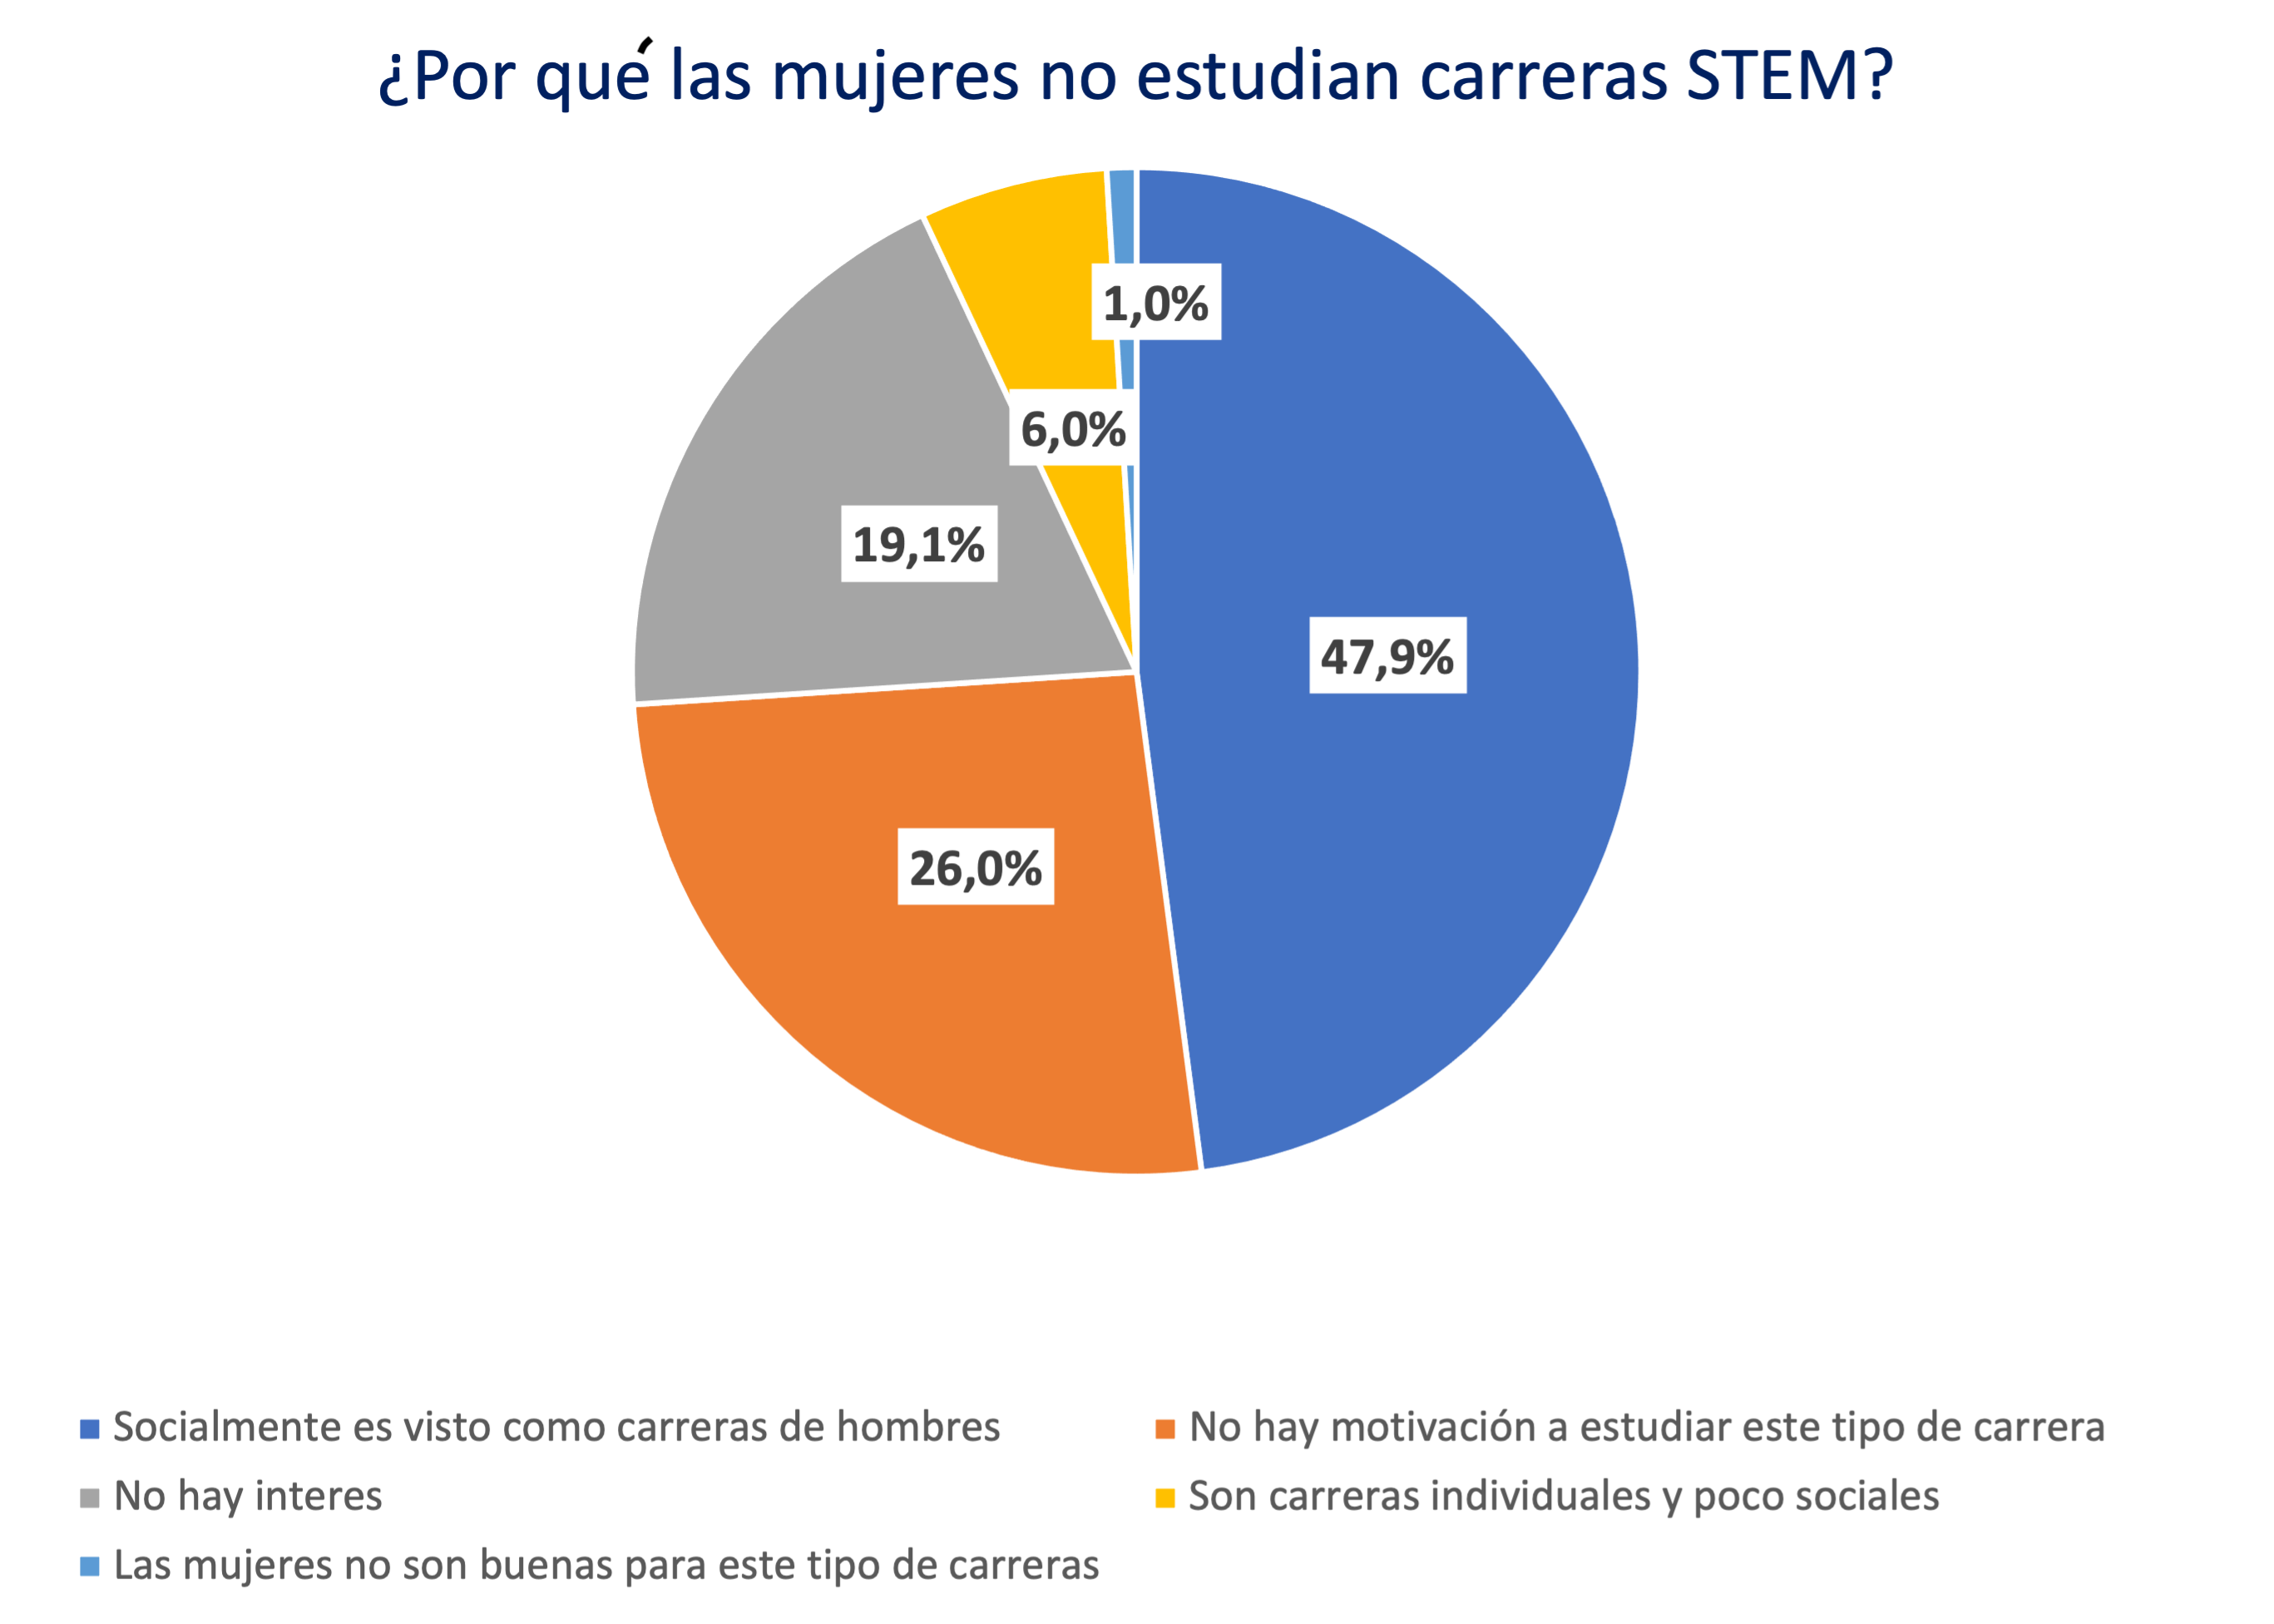
\includegraphics[scale=0.7]{images/figura1.png}
\caption{Respuestas a la pregunta: ¿Por qué las mujeres no estudian carreras STEM?}
\label{fig:1} 
\source{Elaboración propia.}
\end{figure}

Al realizar un análisis por sexo a esta pregunta, del universo que dio como respuesta que estas carreras son vistas como carreras de hombres, el 60,3~\% corresponde a mujeres y solo el 39,7~\% a hombres, algo similar ocurre con las respuestas de que no existen motivaciones para que mujeres estudien carreras STEM y la respuesta que las mujeres no son buenas para estudiar este tipo de carrera ya que del universo que responde el 64,6~\% y 66,7~\% respectivamente son mujeres, en la última respuesta se puede apreciar el menor autoconcepto de las encuestadas con respecto a su capacidad en las áreas de STEM.
Por su parte, el 73,3~\% de los hombres cree que los bajos números de mujeres en este tipo de carreras se debe al poco interés de las mujeres en estas áreas.

La \Cref{fig:2} muestra el porcentaje de hombres y mujeres que seleccionaron cada una de las alternativas.

\begin{figure}[h!]
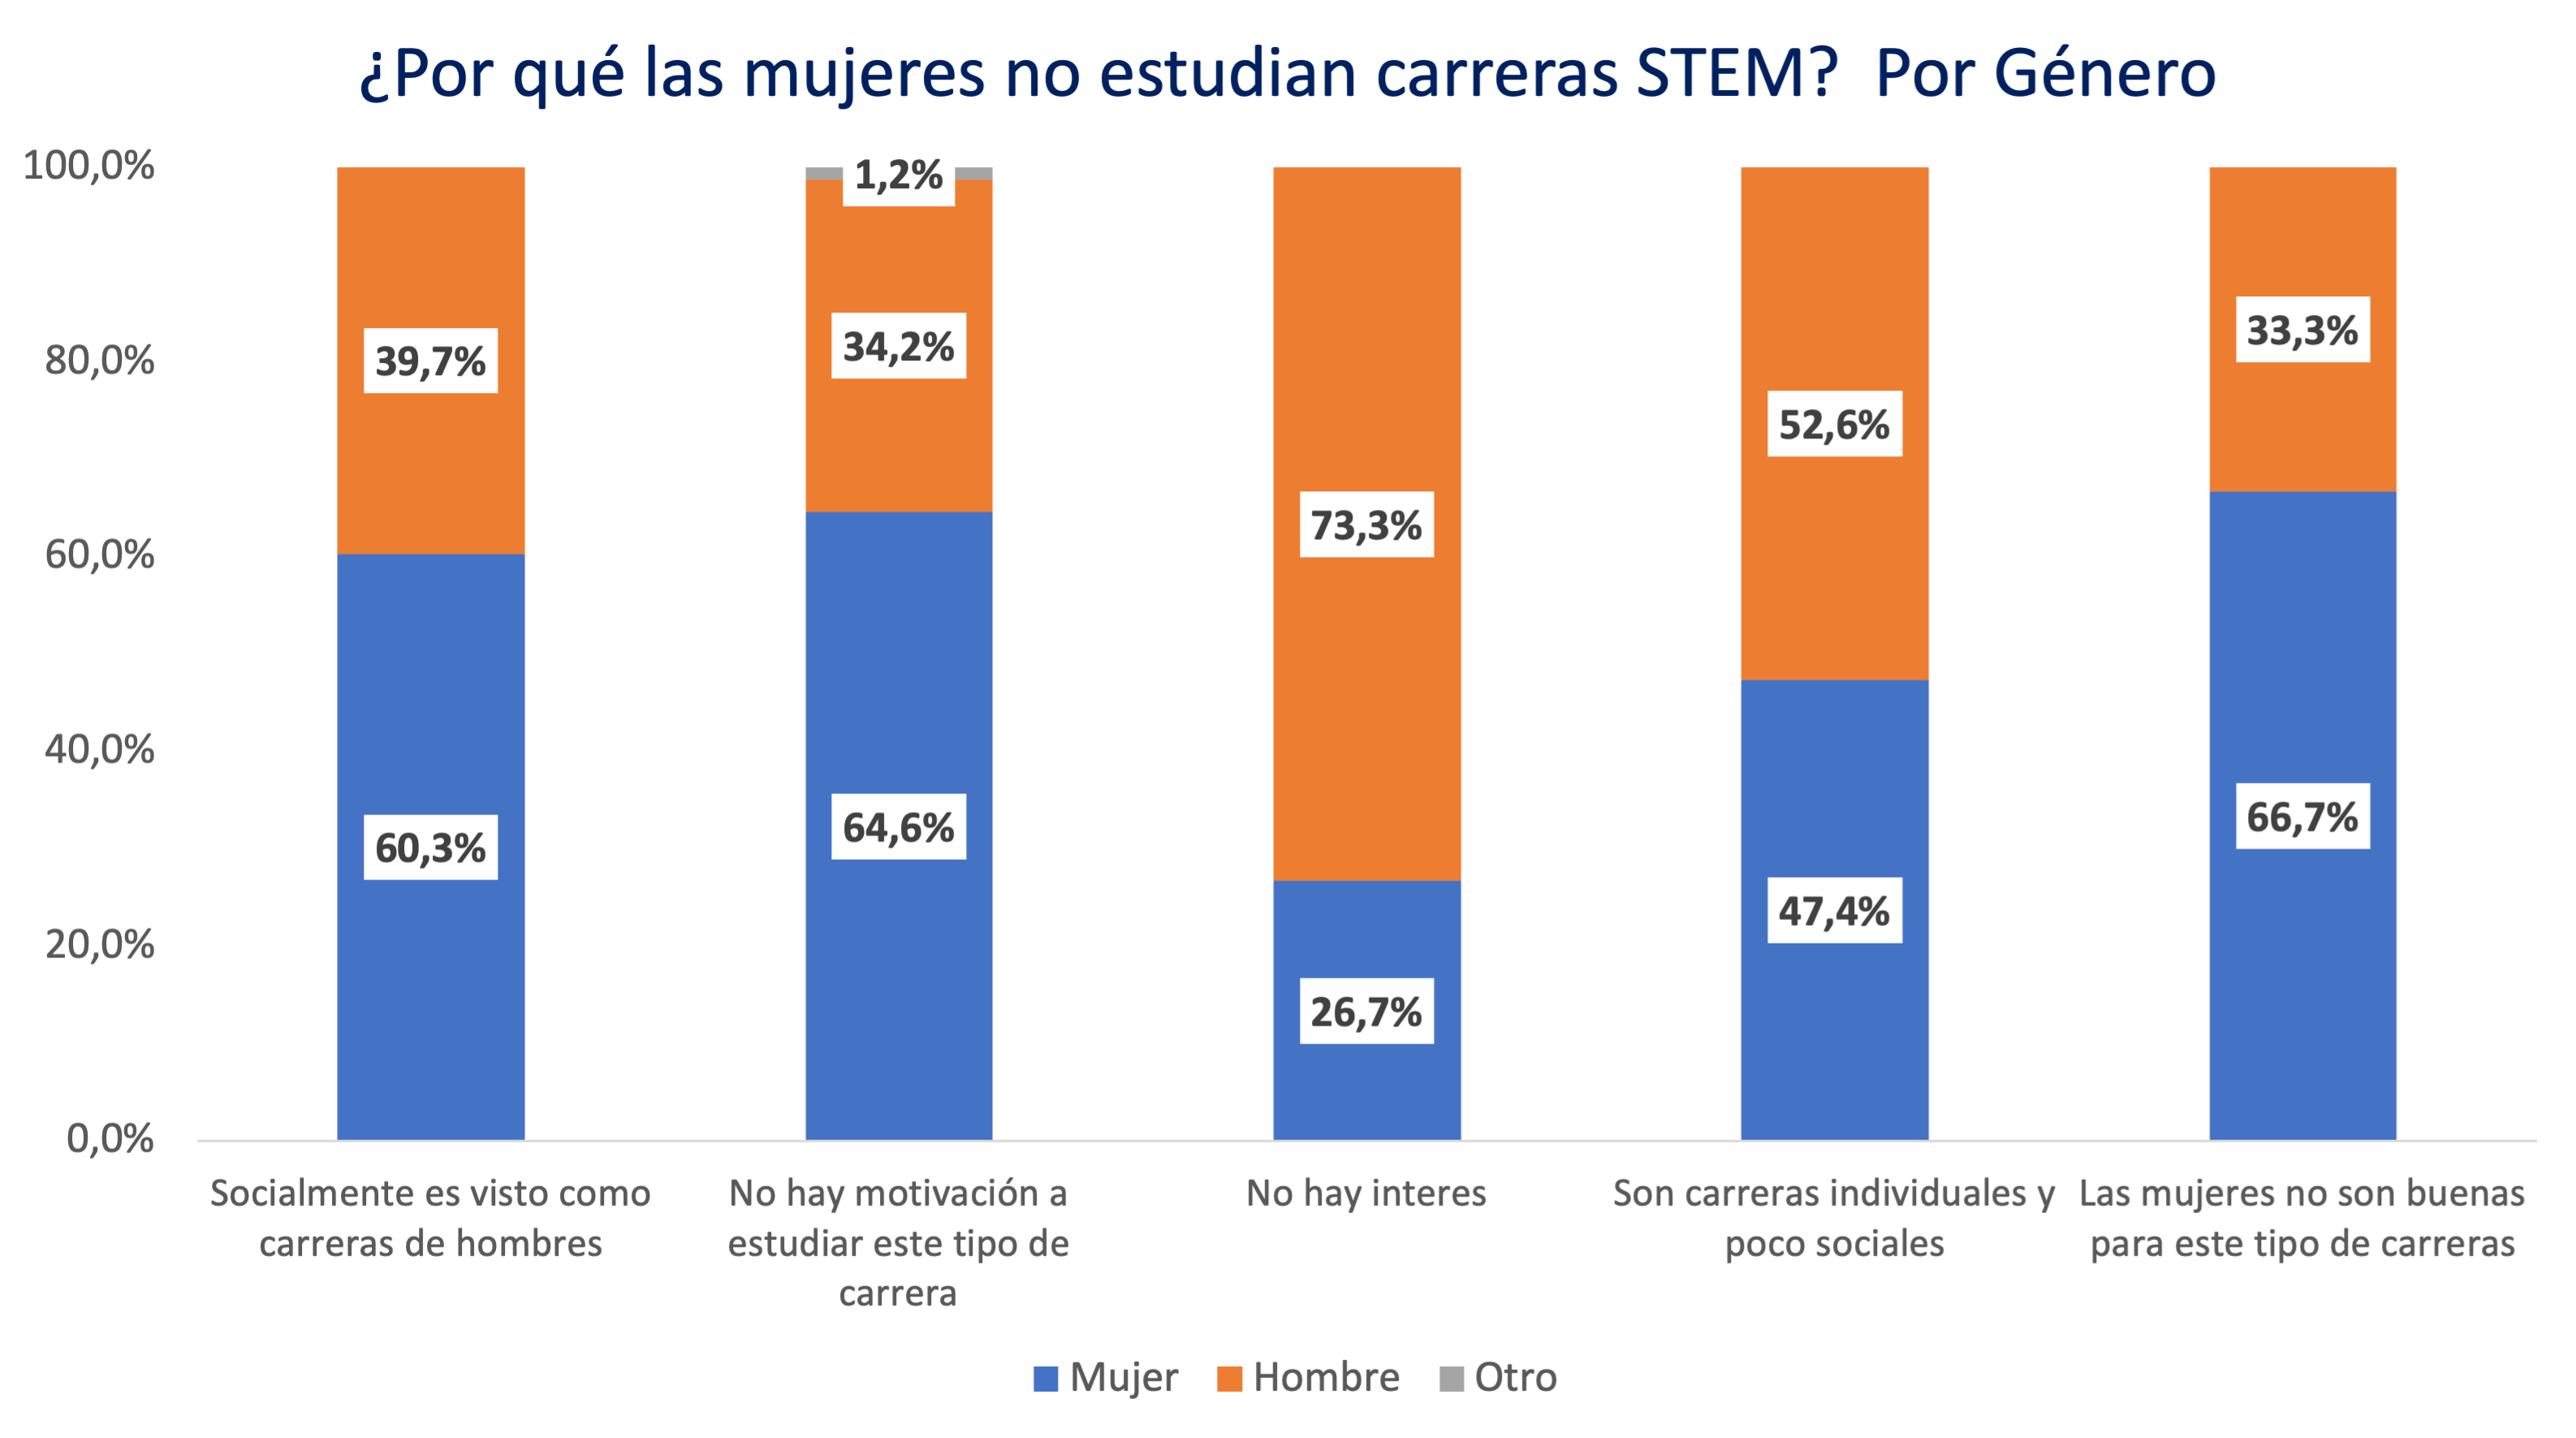
\includegraphics[scale=0.6]{images/figura2.png}
\caption{Respuestas en porcentaje por género a la pregunta: ¿Por qué las mujeres no estudian carreras STEM? }
\label{fig:2}
\source{Elaboración propia.}
\end{figure}

La encuesta intenta indagar sobre el rol de los colegios respecto a potenciar en las mujeres las áreas de STEM. Los resultados no resultan muy alentadores dado que el 65,08~\% de los encuestados considera que los colegios no potencian ni motivan a las niñas a volcarse en estas áreas, la tendencia se refleja tanto en los encuestados que son estudiantes como en aquellos que ya se encuentran trabajando. Al realizar el análisis de esta pregunta por sexo, el 69,36~\% de las mujeres cree que los colegios no potencian a las niñas en las áreas de STEM, en cambio, solo el 46,6~\% de los hombres considera esa premisa.

Al explorar respecto a si una educación familiar machista puede influenciar a las niñas/mujeres a no estudiar carreras del área de STEM, el 66,03~\% de los encuestados responde que la educación familiar influye en la decisión de qué carrera a estudiar. Al extrapolar la pregunta a las instituciones educacionales respecto a si la educación impartida en estos lugares de estudios es machista, el 60,3~\% de los encuestados afirma que la educación recibida es machista; el 70,53~\% de las mujeres considera que existe una educación machista y en cambio solo el 29,6~\% de los hombres considera que la educación tiene un sesgo machista, es decir, el 70,40~\% de los hombres cree que la formación impartida en las instituciones educacionales no es machista, lo que evidencia que hombres y mujeres ven la educación chilena de forma diferente.

A la interrogante de que si existen espacios de colaboración que estimulen el conocimiento en el área de STEM, el 55,56~\% de los encuestados afirma que sí existen, en tanto que un 44,44~\% desconoce
la existencia de tales espacios. Al realizar el análisis por sexo el 54,39~\% de las mujeres cree que no existen espacios de colaboración que estimulen el interés en esta área, en cambio el 67,13~\% de los hombres afirman que estos espacios existen. Al focalizar la pregunta a si existen espacios didácticos que acerquen a las niñas a las área STEM, el 59,68~\% de los encuestados afirma que no existen tales espacios.

Para conocer el impacto de las actividades que realizan diversas universidades chilenas en colegios para motivar a niñas a estudiar carreras STEM, el 78,1~\% de los encuestados afirma que estas actividades contribuyen en el interés de las niñas a estudiar carreras STEM, los hombres valoran más este tipo de actividades para fomentar el interés en las áreas de STEM que las mujeres (85,12~\% v/s 80,64~\%), los estudiantes tienen una mayor valoración de este tipo de actividades que aquellos que están en el mundo laboral (81,64~\% v/s 72,82~\%).

Al preguntar a los encuestados si conocían referentes femeninos en el área de STEM, el 67,94~\% de los encuestados afirma conocer mujeres relacionadas a áreas STEM, solo un 32,06~\% afirma no conocer alguna referente mujer en el área. Conjuntamente, se preguntó si conocían científicas relevantes en el área de STEM, el 56,51~\% de los encuestados afirma conocer al menos una y el 43,49~\% reconoce no conocer a ninguna científica, lo que resulta inquietante dado los grandes avances en esta área que han sido logro de mujeres. Dentro del universo encuestado, los hombres son quienes afirman conocer científicas relevantes en mayor porcentaje con un 60,14~\%, en tanto las mujeres el 53,22~\% afirman conocer alguna científica relevante.

Se pregunto respecto a la autopercepción de las habilidades en las matemáticas, el 83,81~\% de los encuestados responde que manejan un buen autoconcepto, con solo un 16,19~\% de los encuestados no la reconoce, el 88,11~\% de los hombres declara tener una buena autopercepción de sus habilidades matemáticas, el promedio de las mujeres alcanzó un 80,12~\%.

Para la pregunta de si hombres y mujeres tienen las mismas habilidades en matemáticas, el 90,16~\% de la muestra responde que sí, en tanto, solo un 9,84~\% responde negativamente, al reformular la pregunta y plantear si los hombres tienen más habilidades para las matemáticas que las mujeres, el 90.48~\% responde que no, frente a solo un 9,52~\% que piensa que así es. 
Finalmente, se indaga sobre cuáles son las áreas donde las que las mujeres presentan mejor desempeño, la muestra afirma con un 48,08~\% que las áreas donde presentan mejor desempeño las mujeres es indiferente, lo sigue con un 21,47~\% las áreas de ciencias sociales y biología y en tercer lugar con un 6,73~\% las áreas de educación y artes. Las repuestas de las mujeres se inclinan al área de ciencias sociales, biología, en cambio los hombres de la muestra piensan que las mujeres son mejores en las áreas de educación y Artes.

Del análisis detallado y exhaustivo de las resultados de la encuesta, se logro identificar cinco áreas de acción donde resulta relevante poder intervenir proponiendo soluciones, estas áreas se describen en la \Cref{tbl01}.

\begin{table}[htpb]
\centering
\begin{threeparttable}
\caption{Áreas de acción.}
\label{tbl01}
\begin{tabular}{p{\textwidth}}
\toprule
Áreas de acción\\
\midrule
\textbf {Mujeres en cargos de directivos y gerenciales:} Existe una menor Participación de las mujeres en roles gerenciales en las empresas, las medidas implementadas no han sido suficientes, logrando avanzar solo de un 9~\% a un 17~\% en 2020 \cite{DiarioFinanciero2022} \\

\textbf {Mujeres en investigación:} La participación de las mujeres en investigación el 2019 según la \posscite{UNESCO2020} corresponde al 29,3~\%, en Chile este porcentaje aún es menor 22~\%\cite{MinisteriodeCienciasyTecnologias2022}.
 \\

\textbf {Mujer emprendedora:} Según el INE, en el 2017, solo un 38,1~\% de quienes emprenden son mujeres, se debe incentivar a las mujeres a idear y desarrollar emprendimientos tecnológicos \cite{InstitutoNacionaldeEstadisticas2022}  \\

\textbf {Mujer en educación escolar:} Resolver estereotipos de género en la educación es clave, dado que las niñas presentan menor autoconcepto en ciencias y tecnológicas comenzando Educación Primaria y perpetuándose en incrementándose en la Educación Secundaria y Universitaria. De forma generalizada tienen menos confianza en sí mismas en las áreas de ciencia y tecnología en las Escuelas Primarias y Secundarias \cite{Kucuk2020,McGuire2020}
\\
 
\textbf{Mujer en educación Universitaria:} Existen estereotipos en la Educación superior muy marcadas donde se afirma que las mujeres tienen un mayor éxito en las carreras de salud y educación en contrapuesto con carreras STEM \cite{Garcia-Holgado2019,Garcia-Holgado2020}.

\\
\bottomrule
\end{tabular}
\source{Elaboración propia.}
\end{threeparttable}
\end{table}



\subsection{Desarrollo iniciativa Hack4women}

La iniciativa se desarrolló desde el 26 al 28 de agosto 2021, en donde participaron 316 alumnos, 17 docentes, 4 representantes de la Empresa y 2 emprendedoras. En la actividad los alumnos durante tres días trabajan de forma colaborativa para generar soluciones para el área de su interés.

\begin{figure}[h!]
 \centering
 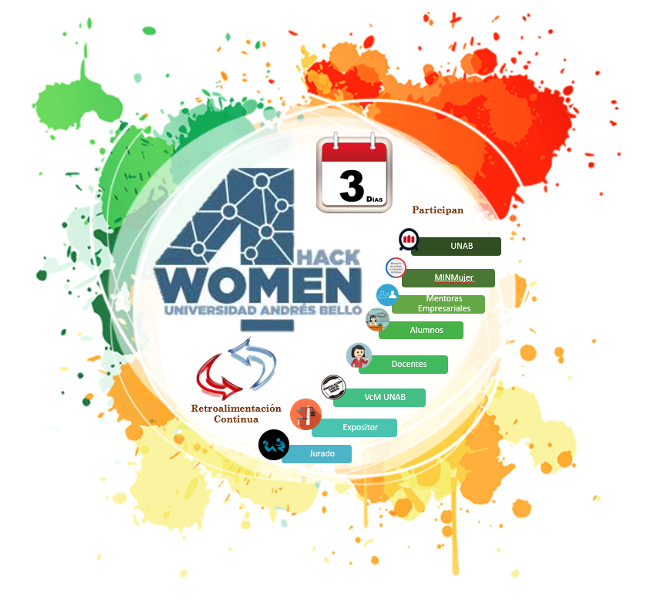
\includegraphics[width=0.85\textwidth]{images/figura3.png}
 \caption{Participantes de iniciativa.}
 \label{fig03}
 \source{Elaboración propia.}
\end{figure}

La iniciativa se contó con la participación y colaboración de distintos entes de la sociedad, donde destacan la secretaría regional ministerial (SEREMI) del Ministerio de la Mujer y Equidad de Género quienes realizaron una exposición y participaron como parte del jurado, emprendedoras destacadas quienes aportaron como mentoras, docentes de la UP, alumnos y la unidad de Dirección de Innovación y Transferencia Tecnológica de la UP. 
Los participantes, se presentan gráficamente en la \Cref{fig03}.

La Dirección de Innovación y Transferencia Tecnológica de la UP tuvo la misión de enseñar a los equipos de alumnos a idear soluciones de valor, empaquetar necesidades y finalmente crear pitch con la solución propuesta, por su parte los docentes asumieron el rol de mentores, que guiaron a los equipos en cada una de estas etapas, el objetivo de su rol fue guiar hacia soluciones viables y de valor que permitieran impactar en las áreas de acción definidas. Para que los equipos pudieran interiorizarse de las experiencias que a diario enfrentas las mujeres en estas áreas, se realizaron una serie de videos donde afectadas relataron sus vivencias en cada una de las áreas de acción. Los equipos pudieron profundizar y empatizar de mejor forma con las afectadas, teniendo una sesión de sesión virtual en donde pudieron conocer y preguntar cuales eran sus necesidades y de qué forma podían mitigarse.
La actividad no solo consistió en desarrollar una solución, sino que, además, la iniciativa busco educar y visibilizar la importancia de temática de género, para este objetivo fueron invitados referentes en el área quienes compartieron experiencias y dieron diversas charlas relacionadas a la temática.

En la primera jornada se invitó a toda la comunidad a asistir, se presentó el resultado de la encuesta ciudadana y se expuso la radiografía de género en la región, posterior a ellos se realizan dos exposiciones de mujeres líderes en tecnología, quienes explicaron las dificultades y complicaciones que debieron enfrentar para llegar a puestos de liderazgo.

La segunda jornada considera una serie de mentorías destacan:Técnicas para definir el propósito de una solución,ideación de una solución,empaquetamiento de ideas, para finalmente, explicar las técnicas para realizar un pitch de éxito. Cada una de las etapas son apoyadas por los docentes de la institución universitaria.. 

Durante la última jornada, los equipos ajustan sus pitch y posteriormente, presentan sus propuestas al jurado, el cual estaba conformado por miembros de la academia, empresa y gobierno, quienes seleccionaron las tres mejores propuestas de solución.

La ruta de las actividad puede ser vista en la \Cref{fig04}.

\begin{figure}[h!]
 \centering
 
\includegraphics[width=0.85\textwidth]{images/figura4.png}
 \caption{Hoja de ruta de la Iniciativa.}
 \label{fig04}
 \source{Elaboración propia.}
\end{figure}

\section{Resultados y discusión}

La actividad entrego como resultado treinta propuestas de solución, de las cuales dieciocho de estas impactan de forma directa a los ámbitos de acción definidos.
En la \Cref{tbl02}, se muestras seis iniciativas propuestas de los grupos de trabajo.

\begin{table}[htpb]
\centering
\begin{threeparttable}
\caption{Iniciativas destacadas.}\label{tbl02}
\begin{tabular}{p{\textwidth}}
\toprule
Iniciativas\\ 
\midrule
\textbf{Poderosas} Aplicación móvil que tiene por objetivo enseñar y visibilizar el rol de las mujeres en el área de STEM, mediante actividades lúdicas y de diversión.\\ 
\textbf {Inspira U } Creación de comunidad que visibilice los proyectos de investigación desarrolladas por mujeres y fomente el desarrollo de líderes femeninos.\\ 
\textbf {Investigadoras STEM:} Portal web que concentre a todas las investigadoras a nivel nacional en el área de STEM, junto a sus publicaciones y áreas de interés, el fin es generar una comunidad de investigadoras a nivel nacional donde puedan generar redes y compartir conocimientos.\\ 
\textbf {Emprendedoras en tecnología: } Portal web que concentre todos los fondos concursables, beneficios entregados por el estado, patrocinios, seminarios y cursos  a nivel nacional e internacional donde sea posible postular, adicionalmente el portal entregará tips que ayuden a las mujeres emprendedoras\\ 
\textbf {Adopta a una ahijada:}  Iniciativa que busca generar el lazo entre las universitarias y las alumnas de colegio motivadas e interesadas por el área de STEM.\\ 
\textbf {Mentoras:} Portal web que permita vincular a alumnas universitarias y mujeres de empresa o emprendimiento, con el fin de generar proyectos y trabajos colaborativos en el área de STEM.\\
\bottomrule
\end{tabular}
\source{Elaboración propia.}
\end{threeparttable}
\end{table}

La iniciativa de “Hack4women”, logró convocar a alumnos de cuatro programas de estudios de la Facultad de Ingeniería y todas las sedes donde la UP tiene presencia en Chile.

La iniciativa no solo permitió tener una radiografía de la mirada de la ciudadanía respecto a esta temática, sino que además permitió educar y visibilizar por medio de ponencias y vivencias sobre la importancia de crear una sociedad sin sesgo de género. 

Relevante fue participación de la academia, empresa y gobierno quienes aportaron a la creación de un espacio de co-creación, colaboración y reflexión en torno a las diversas aristas relacionadas a la brecha de género en STEM.

\section{Conclusiones}\label{sec-organizacao}

La iniciativa permitió convocar a diversos actores de la sociedad como son: academia, industria y Estado, quienes dieron vida a un espacio de colaboración y reflexión en torno la brecha de género en STEM. 

Fue posible obtener la visión de la ciudadanía respecto a las principales dificultades y dolores que enfrentan las mujeres desde la infancia hasta la vida adulta en el área de STEM, de forma adicional se logro identificar cinco áreas de acción claras sobre las que hay que centrar los esfuerzos para mitigar la brecha de género en el área STEM.
Treinta propuestas llegan a término de las cuales dieciocho impactan de forma directa a una de las cinco áreas de acción de definidas, logrando mitigar las brechas en esta área.

La próxima etapa considera la implementación de las propuestas de solución de forma que la ciudadanía se vea beneficiada y se avance en la reducción de brechas de género en STEM.

Se desea realizar una nueva versión a nivel internacional, donde alumnos de distintos países y universidades trabajen de forma conjunta en propuestas de soluciones que reduzcan la brecha de genero en STEM. Adicionalmente se desea invitar a participar a organismo privados y públicos de diversos países quienes aporten su mirada a soluciones en esta temática. En Chile se desea generar contacto con el ministerio de Ministerio de Ciencia, Tecnología, Conocimiento e Innovación \cite{MinisteriodeCienciasyTecnologias2022},  quienes pueden ser referentes en el trabajo de reducir las brechas en STEM para las mujeres.

\printbibliography\label{sec-bib}
% if the text is not in Portuguese, it might be necessary to use the code below instead to print the correct ABNT abbreviations [s.n.], [s.l.]
%\begin{portuguese}
%\printbibliography[title={Bibliography}]
%\end{portuguese}


%full list: conceptualization,datacuration,formalanalysis,funding,investigation,methodology,projadm,resources,software,supervision,validation,visualization,writing,review
\begin{contributors}[sec-contributors]
\authorcontribution{Giannina Costa-Lizama}[conceptualización, supervision]
\authorcontribution{Lilian San-Martin}[datacuration, formalanalysis, funding, methodology, resources, validation]
\authorcontribution{Oscar Pinto}[conceptualization, resources, validation]
\authorcontribution{Gustavo Gatica}[datacuration, formalanalysis, methodology, projadm, software, supervision, review]
\end{contributors}

\end{document}

